\documentclass{article}

% Language setting
% Replace `english' with e.g. `spanish' to change the document language
\usepackage[portuguese]{babel}

% Set page size and margins
% Replace `letterpaper' with `a4paper' for UK/EU standard size
\usepackage[letterpaper,top=2cm,bottom=2cm,left=3cm,right=3cm,marginparwidth=1.75cm]{geometry}

% Useful packages
\usepackage{amsmath}
\usepackage{graphicx}


\title{MAP2212 - Exercício de Programação 3}
\author{Lucas Panfilo Donaire - 12556552}

\begin{document}
\maketitle

\newcommand{\PR}[1]{\ensuremath{\left[#1\right]}}
\newcommand{\PC}[1]{\ensuremath{\left(#1\right)}}
\newcommand{\chav}[1]{\ensuremath{\left\{#1\right\}}}

\begin{abstract}
Comparando geradores de números pseudo aleatórios com números quasi aleatórios para integrações usando métodos de Monte Carlo,
\end{abstract}

\section{Introdução}
\subsection{EP2}
No EP2, usamos alguns métodos para estimar a integral de f(x), dada por: \\
$f(x) = e^{-0.57892819x}\times cos(0.47410024895x)$ \\

Os métodos usados foram: "crude", "hit or miss", "importance sampling" e "control variate". Usamos números pseudo aleatórios para estimar a integral. Nesse EP3, nosso objetivo é comparar os números pseudo aleatórios com os números quasi aleatórios.

\section{Geradores de Números aleatórios}
Computadores não conseguem simular eventos realmente aleatórios, mas conseguem gerar sequências de números (de um conjunto finito ou intervalo da reta) aproximadamente independentes e que não afetam o resultado quando usados em métodos de Monte Carlo. Temos alguns métodos para gerar esses números.

\subsection{Pseudo-aleatoriedade}
Sequências pseudoaleatórias tipicamente exibem aleatoriedade estatística enquanto estão sendo geradas por um processo inteiramente determinístico. Um processo muito usado em estatística para isso são os  \textbf{Geradores congruenciais lineares}:
São gerados por sequências da forma
\[
X_{n+1} = (a \cdot X_n + c) \mod m
\]
Vantajosos por sabermos período máximo = $a \cdot m$, e gerarem números em [0,m).

\begin{figure}[ht]
\centering
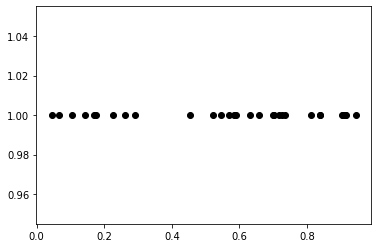
\includegraphics[width=0.4\textwidth]{random_1.png}
\caption{\label{fig:random_1} pontos pseudo aleatórios na reta }
\end{figure}

\newpage

\subsection{Números quasi-aleatórios e sequências de Halton-Hammersley}
Sequências quasi-aleatórias são construídas a partir de uma base b, e preenchem o intervalo selecionado de uma forma aproximadamaente uniforme. São determinísticas, geradas por reversão de bits, mas também podem ser consruídas de outras formas por algorítmos aritméticos.

\begin{figure}[ht]
\centering
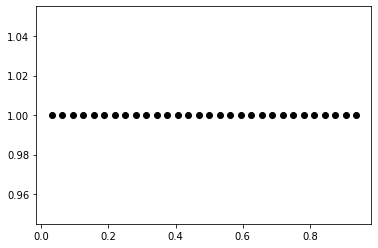
\includegraphics[width=0.3\textwidth]{halton_1.png}
\caption{\label{fig:halton_1} pontos quasi aleatórios na reta }
\end{figure}


\begin{figure}[ht]
\centering
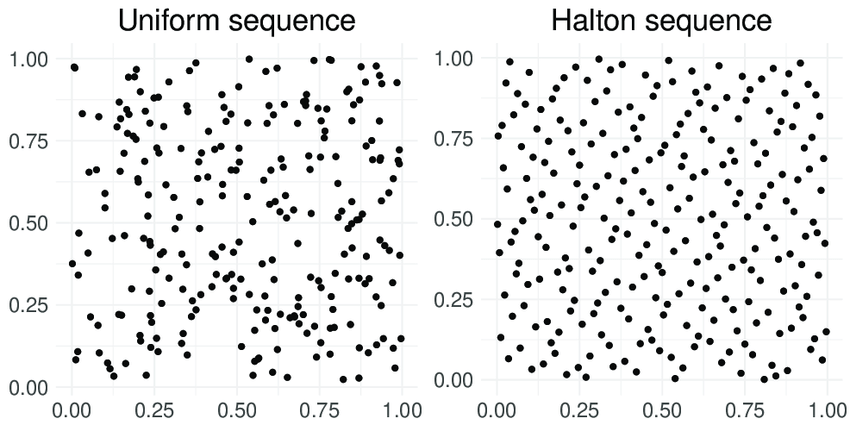
\includegraphics[width=0.6\textwidth]{uniforme_halton.png}
\caption{\label{fig:uniforme_halton} comparação de pontos no quadrado unitário }
\end{figure}


Fizemos a seguinte função para gerar uma sequência de Halton com base b e tamanho n:
\begin{figure}[ht]
\centering
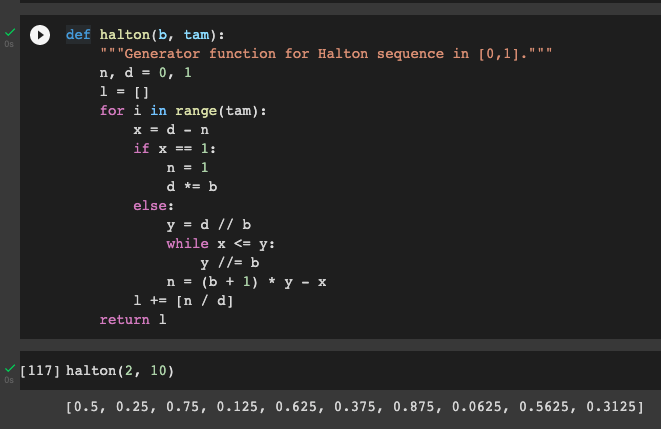
\includegraphics[width=0.5\textwidth]{halton_function.png}
\caption{\label{fig:halton_funciton} função geradora de sequências de halton acompanhada de exemplo na base 2 (igual ao exemplo do professor)  }
\end{figure}


\subsection{Alguns resultados que iremos usar}
\subsubsection{Somas da Integral de Darboux}

A integral de Darboux é equivalente à de Riemann e construída a partir de duas somas, uma soma inferior que é sempre menor que a integral, e uma soma superior que é sempre maior. Definição: 

Seja $P = \PC{x_0, x_1,..., x_n}$ uma partição de \PR{a,b}. 
\\
Seja $M_i = sup(f(x)), x \in [x_{i-1}, x_i]$, para i = 1,2,..,n \\
Seja $m_i = inf(f(x)), x \in [x_{i-1}, x_i],$ para i = 1,2,..,n \\
A soma Darboux superior de f em relação a P é: 

\[
U_{f,P} = \sum_{i=1}^{n} (x_i - x_{i-1})M_i 
\]
E a soma Darboux inferior de f em relação a P é:
\[
L_{f,P} = \sum_{i=1}^{n} (x_i - x_{i-1})m_i 
\]
Temos que, para qualquer partição P de (a,b), vale:
\[
U_{f,P} \leq \int_{a}^{b} f(x)dx \leq  L_{f,P}
\]
Isso será útil para calcular limitantes superiores e inferiores da integral que queremos estimar.


\begin{figure}[ht]
\centering
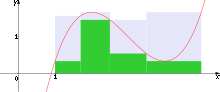
\includegraphics[width=0.35\textwidth]{darboux.jpeg}
\end{figure}



\section{Sobre a estimação da integral}
Pela intuição, parece razoável achar que a estimativa integral converge mais rápido para o valor desejado quando usamos pontos que preenchem mais uniformemente a reta, então acreditamos que os números quasi-aleatórios se sairão melhores. Além disso, apesar de não medirmos a variância das nossas sequências de Halton, medimos sua discrepância, que cresce de forma muito menor que a variância dos números pseudo-aleatórias (é mais homogênea).

\subsection{Cuidados com sequências de Halton}
No último EP, vimos os métodos para estimar a integral. Três deles usavam números aleatórios, e um deles usava pontos aleatórios (hit or miss)

Para os três que usam pontos aleatórios, só basta trocar o gerador de congruência linear pelas sequências de halton (com o cuidado do número de pontos ser bem superior à base para os pontos não ficarem presos numa região da reta: ver Figura abaixo)

\begin{figure}[ht]
\centering
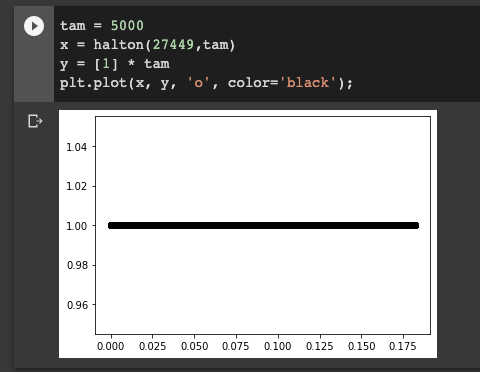
\includegraphics[width=0.4\textwidth]{falha_halton.png}
\caption{\label{fig:falha} gerando uma sequência de 5000 números com base 27449 - ficamos presos ao intervalo [0, 0.175]  }
\end{figure}

Já no caso do método hit or miss, temos que tomar cuidado: se usarmos a mesma base para gerar x e y do ponto aleatório (x,y), só teríamos elementos na diagonal principal (se usássemos o mesmo índice para x e y) ou formando um padrão muito específico (quando trocamos o índice): Ver figura abaixo

\begin{figure}[ht]
\centering
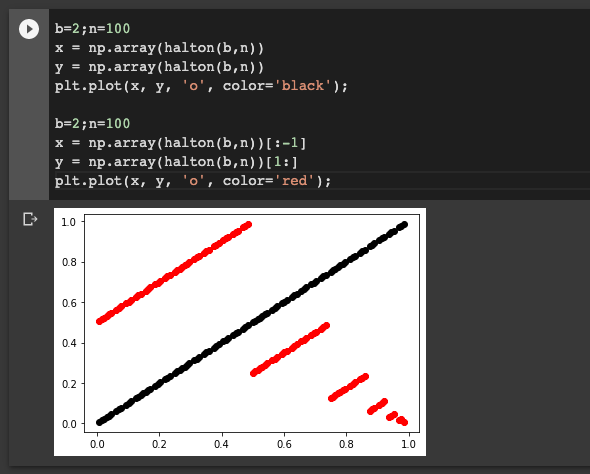
\includegraphics[width=0.5\textwidth]{falha2.png}
\caption{\label{fig:falha2} Em preto, mesma base e mesmo indice; em preto, mesma base e indíces diferentes  }
\end{figure}

E mesmo se mudássemos as bases, se elas tiverem um quociente próximo de 1, também falham em preencher o quadrado uniforme.

\begin{figure}[ht]
\centering
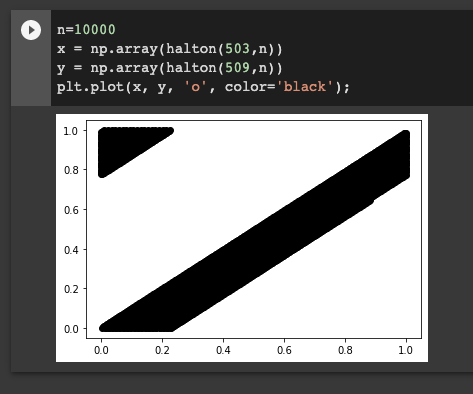
\includegraphics[width=0.5\textwidth]{falha3.png}
\caption{\label{fig:falha4} 10000 pontos (x,y) tal que x era uma sequencia de halton com base 503, e y com base 509  }
\end{figure}


\subsection{Testando a convergência e erro}
Como nosso objetivo é comparar métodos e não mais estimar o valor exato da integral, usamos as somas de Darboux para estimar um intervalo que contém nossa integral, e usar isso para calcular o erro.

\begin{figure}[ht]
\centering
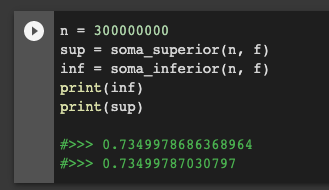
\includegraphics[width=0.5\textwidth]{inf_sup.png}
\caption{\label{fig:infsup} intervalo [inf, sup] contém o verdadeiro valor da integral  }
\end{figure}

Criamos uma função de erro da seguinte forma:
se o valor estimado estivesse entre [inf,sup], erro=0; se o valor fosse maior que sup medíamos o erro relativo a sup; se o erro fosse menor que inf, medíamos o erro relativo a inf. Assim, dados base b e número de pontos n, conseguíamos medir a qualidade da nossa estimativa. A partir disso, fizemos uma função de teste que se comportava da seguinte maneira: Rodava a função de estimativa com n pontos com os 30 primeiros números primos de base (Obs: na hit or miss, uma base foi 2 e a outra foi mudando entre os 29 primeiros primos maiores que 2) , e calculava a média dos erros e quantas estimativas estavam entre $[0,9995 \cdot inf , 1,0005 \cdot sup]$. Iterativamente, aumentando o n, quando todos erros estivessem dentro da margem, parávamos.
Achamos os seguintes resultados:

\subsection{Resultados - Estimação}
Criando um data frame com os resultados dessa função teste e algumas manipulações, temos:
\begin{figure}[ht]
\centering
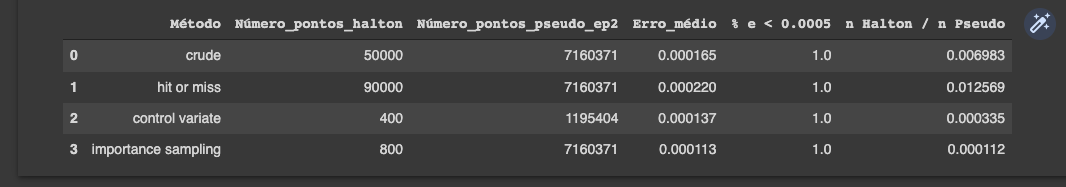
\includegraphics[width=1\textwidth]{results.png}
\end{figure}

Esse é um resultado impressionante: todos os métodos usaram menos de 2\% dos pontos do EP anterior. O pior método usa 90 mil pontos, e o melhor usa impressionantes 400 pontos!


\subsection{Resultados - Tempo}
Ao fazer uma função para rodar os estimadores do EP2 e EP2 e medir o tempo, encontramos:

\begin{figure}[ht]
\centering
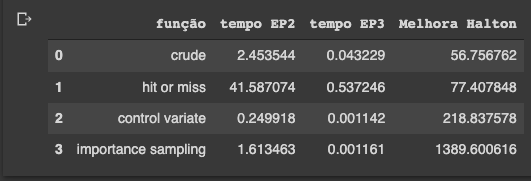
\includegraphics[width=1\textwidth]{comparacao.png}
\caption{\label{fig:comparacao} tempos em segundo para rodar o código. melhora halton é o quociente dos tempos dp EP2 pelo EP3  }
\end{figure}

\section{Conclusão}
Conclusão: como nossa intuição esperava, sequências de Halton-Hammersen são muito superiores às pseudo-aleatórias na estimação de integral, reduzindo muito o tempo e a quantidade de pontos usada.

\section{Referências}
Bussab \& Morettin - Estatística Básica, $6^a$ edição. Editora Saraiva, 2009.
\\
https://stringfixer.com/pt/Darboux\_integral
\end{document}
